\documentclass{article}

\usepackage{graphicx}
\usepackage{listings}

\begin{document}

\begin{center}

\includegraphics[width=3cm]{iiitb_logo.png}

\vspace{0.4cm}

IIIT Bangalore

\vspace{0.3cm}

Name: Srinidhi A

ID: COMETFWC053

\vspace{0.5cm}

Question 13

\end{center}

\section*{Question}

The complete set of only those logic gates designated as universal gates is

\begin{tabular}{ll}
(a) & NOT, OR and AND \\
(b) & XNOR, NOR and NAND \\
(c) & NOR and NAND \\
(d) & XOR, NOR and NAND \\
\end{tabular}

\section*{Analysis}

Universal gates are gates that can implement any Boolean function.

For two inputs $A$ and $B$

NAND gate output

$NAND = \overline{A \cdot B}$

NOR gate output

$NOR = \overline{A + B}$

Using only NAND gates or only NOR gates we can construct AND, OR and NOT gates.  
Therefore NAND and NOR are called universal gates.

Correct option: (c) NOR and NAND.

\section*{Python Code}

\begin{lstlisting}
import numpy as np
import matplotlib.pyplot as plt

A = np.array([0,0,1,1])
B = np.array([0,1,0,1])

NAND = 1 - (A & B)
NOR = 1 - (A | B)

print("A B NAND NOR")

for i in range(4):
    print(A[i], B[i], NAND[i], NOR[i])

x = np.arange(4)

plt.step(x,A,where='post',label='A')
plt.step(x,B,where='post',label='B')
plt.step(x,NAND,where='post',label='NAND')
plt.step(x,NOR,where='post',label='NOR')

plt.grid()
plt.legend()
plt.savefig("graph.png")
plt.show()
\end{lstlisting}

\section*{Graph}

\begin{center}

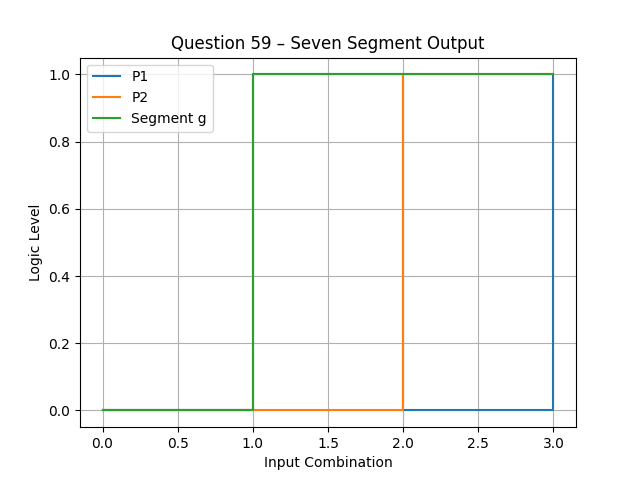
\includegraphics[width=10cm]{graph.png}

\end{center}

\section*{Conclusion}

From the truth table and the graph it is clear that NAND and NOR gates can implement all basic logic gates. Hence they are universal gates.

\end{document}
